\documentclass[12pt]{mwart}

\usepackage{polski}
\usepackage[utf8]{inputenc}
\usepackage{mathtools,amsthm,amssymb,icomma,upgreek,xfrac, graphics, scrextend}
\usepackage{amsmath}
\usepackage{graphicx}
\usepackage{float}

\newtheorem{def2}{DEF.}

\begin{document}
	
	\begin{center}
		{\Large\textbf{Komputerowa analiza szeregów czasowych}}
	\end{center}
	\begin{center}
		Raport: \textbf{2}
	\end{center}
	
	\noindent Temat sprawozdania  \textbf{Wykorzystanie poznanych metod służących do analizy zależności liniowej dla wybranych danych rzeczywistych.
	} \\
	Nazwisko i Imię prowadzącego kurs \textbf{Inż. Justyna Witulska} 	\newline\newline
	
	
	\noindent\begin{tabularx}{\textwidth}{|X |X|}
		\hline
		Wykonawca: & \\\hline
		\begin{center}
			Imię i Nazwisko,\\ nr indeksu
		\end{center} &  \begin{center}
			Adrianna Ziobroniewicz, 262227\\
			Anna Zadka, 262226
		\end{center}\\\hline
		Wydział & Wydział matematyki, W13 \\\hline
		Termin zajęć: & Środa, $7^{30}$\\\hline
		Numer grupy ćwiczeniowej & T00-79c \\\hline
		Data oddania sprawozdania: & \today \\\hline
		\textbf{Ocena końcowa} &\\\hline
		
	\end{tabularx}\newline\newline
	
	
	
	\newpage
	\tableofcontents
	\newpage
	
	

\section{Wstęp}
\subsection{Wizualizacja danych}


\newpage
\section{Przygotowanie danych do analizy}
\subsection{Zbadanie jakości danych}
Jak wiadomo miasto, które wybraliśmy do analizy to Warszawa. Nasze dane dotyczące dat były rozdzielone, więc zajęliśmy się skonstruowaniem pełnej daty.Do analizy bierzemy średnią temperaturę na dany dzień. Temperatury są podane w stopniach Farenheita, aby były dla nas przyjazne to zamienimy je na stopnie Celsjusza i zaokrąglimy do jednego miejsca po przecinku. \\
Sprawdzamy czy w zbiorze znajdują się jakieś wartości nieznane (NaN), jednakże takich nie ma.\\
Kolejna weryfikacja to powtarzalność indeksów. Taką sytuację zauważamy w grudniu 2015 roku. \\
\begin{figure}[h]
	
	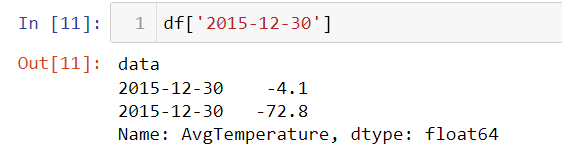
\includegraphics[width=10cm]{indeks.png}
	\caption{2 indeksy powtarzające się zanotowane 30 grudnia 2015 roku}
\end{figure}

Temperatura -72.8 stopnia jest bez dwóch zdań błędem pomiarowym, więc zajmiemy się jego usunięciem. Pozostała nam tylko jedna temperatura, ta poprawna. W ramach dalszej weryfikacji poprawności zbioru zbadamy obecność wartości odstających (outlierów) za pomocą metryki z-score. Określa ona jak daleko nasz wartości znajdują się od standardowych wartości w tym zbiorze. Im większy z-score tym bardziej można podejrzewać, że dana próbka może być outlierem.\\
\begin{figure}[h]
	
	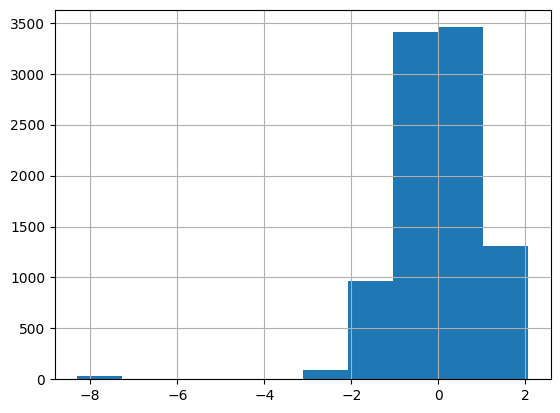
\includegraphics[width=8cm]{outlier.png}
	\caption{2 indeksy powtarzające się zanotowane 30 grudnia 2015 roku}
\end{figure}
\newpage
Większość próbek zawiera się w przedziałach od -3 do 2. Jest to standardowy zakres, który nie powinien budzić naszych obaw. Sprawdźmy, co to są za próbki, które mieszczą się w wartościach poniżej -4.\\
\begin{figure}[h]
	
	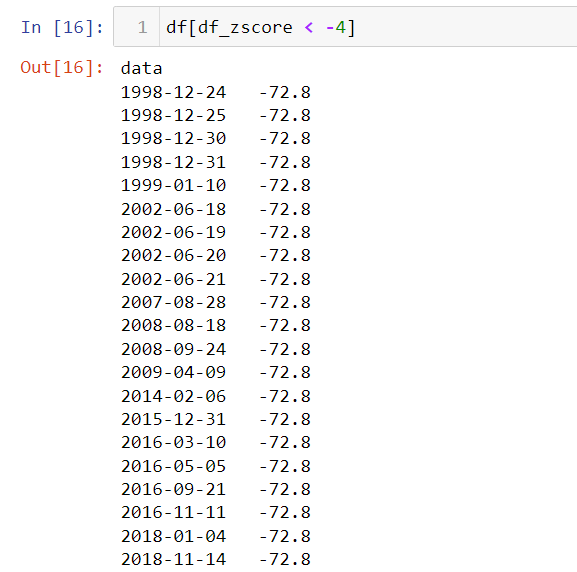
\includegraphics[width=10cm]{outlier1.png}
	\caption{Indeksy poniżej -4 stopni zanotowane w 2015 roku}
\end{figure}

Widzimy wyraźnie, że jest to ta sama wartość, którą usuwaliśmy już wyżej. Jest to zatem błąd w pomiarach. Tym samym każdą z tych wartości usuniemy, a puste pola uzupełnimy wartości 'ffill'' czyli wartością poprzednią. Tym samym jeśli informacja z np. 15 maja zostanie usunięta to za pomocą frontfill zostanie ona uzupełniona wartością z 14 maja. Jest to bezpieczny sposób uzupełniania informacja, gdyż można zakładać, że temperatura w sąsiadujących dniach jest zbliżona do siebie i dokonując takiego uzupełnienia nie przekłamujemy znacząco rzeczywistej informacji.\\
Nasz zbiór został sprawdzony pod wzlędem braków i outlierów. Możemy przejść do dalszej analizy. Na początek znacząco zmniejszymy nasz zbiór robiąc resampling miesięczny, czyli dane dzienne zamienimy na miesięczne w ten sposób, że weźmiemy średnią temperaturę ze stycznia, następnie średnią temperaturę z lutego itd.\\


Następnie dokonamy podziału zbioru na dwa: treningowy oraz testowy. Do treningowego użyte zostaną lata od 1995 do 2017, a na zbiór testowy przeznaczymy ostatnie dwa i pół roku\\
\newpage
\large\textbf{Wykresy ACF oraz PACF dla surowego szeregu}\\

\begin{minipage}{\linewidth}
	\centering
	\begin{minipage}{0.45\linewidth}
	\begin{figure}[H]
		\includegraphics[width=4cm]{treningowy.png}
		\caption{Indeksy poniżej -4 stopni zanotowane w 2015 roku}
	\end{figure}
	\end{minipage}
	\hspace{0.05\linewidth}
	\begin{minipage}{0.45\linewidth}
		\begin{figure}[H]
			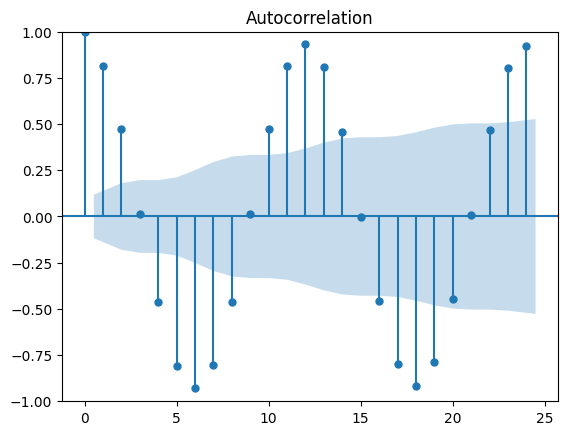
\includegraphics[width=4cm]{acf.png}
			\caption{This is the first figure}
		\end{figure}
	\end{minipage}
	\hspace{0.05\linewidth}
	\begin{minipage}{0.45\linewidth}
		\begin{figure}[H]
			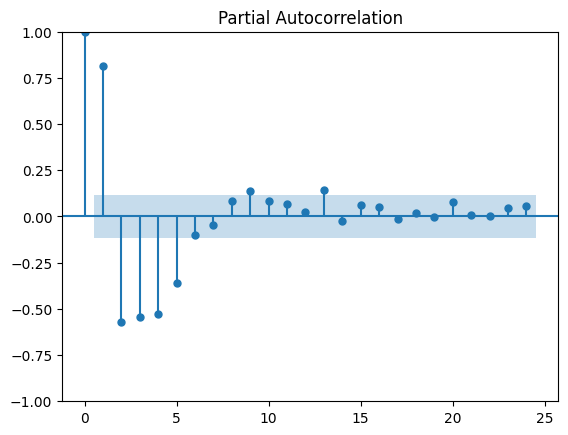
\includegraphics[width=4cm]{pacf.png}
			\caption{This is the second figure}
		\end{figure}
	\end{minipage}
\end{minipage}
\\

\noindent \textbf{Wzór ACF, inaczej funkcja autokoleracji:}
$$ corr(X_t, X_s) = \frac{ \gamma_x(t,s)}{\sqrt{\gamma_x(t,t) \gamma_x(s,s)}} = \rho_x(X_t, X_s).$$
Przy przesunięciu k jest to korelacja między wartościami szeregu oddalonymi o k przedziałów od siebie.\\


\noindent \textbf{Wzór PACF, inaczej cząstkowa funkcja autokoleracji:}
$$ X_t = \phi_0 + \phi_1 X_t-1 + ... + \phi_k X_t-k + Z_t,$$
gdzie ${Z_t} \sim WN(0, \sigma^2).$\\
Przy przesunięciu k jest to korelacja między wartościami szeregu oddalonymi o k przedziałów od siebie, z jednoczesną rejestracją wartości z przedziałów znajdujących się pomiędzy.
\newpage

\large\textbf{Test ADF weryfikujący hipotezę o niestacjonarności dla surowych danych - Augmented Dickey-Fuller Test}\\
\\
Test $ADF$ jest zasadniczo testem istotności statystycznej. Oznacza to, że istnieje testowanie hipotez, które jest związane z hipotezą zerową i alternatywną, w wyniku czego obliczana jest statystyka testowa i podawane są wartości $p$ - z tej statystyki można wywnioskować czy dany szereg jest stacjonarny. \\
$ADF$ jest to rozszerzona wersja Dickeya-Fullera. Rozszerza równanie testy o proces regresji wysokiego rzędu w modelu. Hipoteza zerowa jest jednak taka sama jak przy teście Dickeya-Fullera. Czyli $H_0 = \alpha =1 $. Hipoteza ta zakłada obecność pierwiastka jednostkowego($alpha=1$), otrzymana wartość $p$ powinna być mniejsza niż poziom istotności, aby móc odrzucić hipotezę zerową - tym samym wnioskują, że szereg jest stacjonarny. \\
\begin{figure}[h]
	
	\includegraphics[width=10cm]{test.png}
	\caption{Indeksy poniżej -4 stopni zanotowane w 2015 roku}
\end{figure}

Wartość p == 0.07 nie jest mniejsza niż 0.05 więc nie możemy odrzucić hipotezy zerowej. Tym samym stwierdzamy, że szereg jest niestacjonarny.\\

\newpage
\large\textbf{Wykresy ACF oraz PACF dla uzyskanego szeregu}

\begin{minipage}{\linewidth}
	\centering
	\begin{minipage}{0.45\linewidth}
		\begin{figure}[H]
			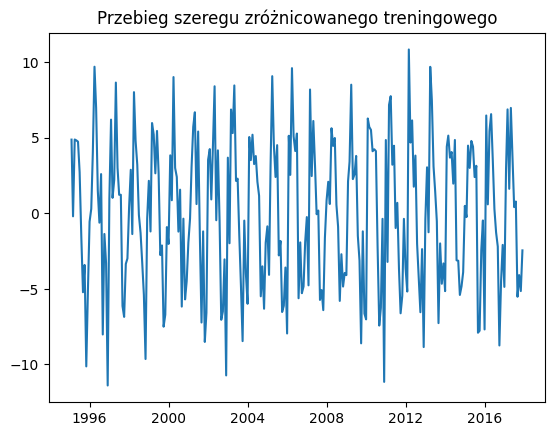
\includegraphics[width=4cm]{nowe.png}
			\caption{Indeksy poniżej -4 stopni zanotowane w 2015 roku}
		\end{figure}
	\end{minipage}
	\hspace{0.05\linewidth}
	\begin{minipage}{0.45\linewidth}
		\begin{figure}[H]
			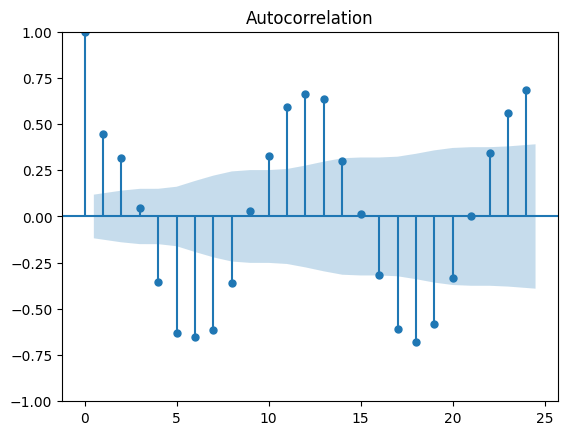
\includegraphics[width=4cm]{acf1.png}
			\caption{This is the first figure}
		\end{figure}
	\end{minipage}
	\hspace{0.05\linewidth}
	\begin{minipage}{0.45\linewidth}
		\begin{figure}[H]
			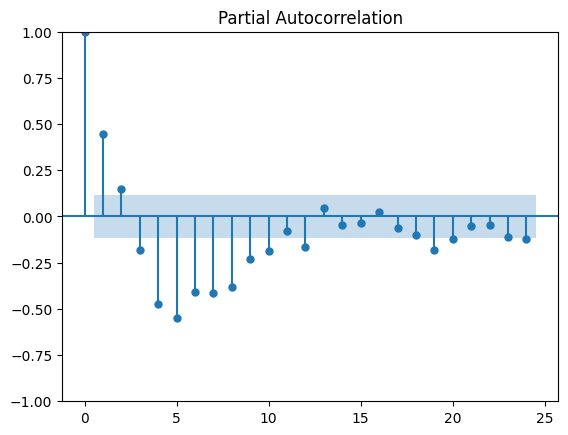
\includegraphics[width=4cm]{pacf1.png}
			\caption{This is the second figure}
		\end{figure}
	\end{minipage}
\end{minipage}

\textbf{Test ADF weryfikujący hipotezę o niestacjonarności dla uzyskanego szeregu - Augmented Dickey-Fuller Test}

\begin{figure}[h]
	
	\includegraphics[width=10cm]{test1.png}
	\caption{Indeksy poniżej -4 stopni zanotowane w 2015 roku}
\end{figure}

Wartość p-value spadła do bardzo małej wartości. Oznacza to, że tym razem otrzymany szereg jest szeregiem stacjonarnym.





\newpage
\section{Modelowanie danych przy pomocy ARMA}
\textbf{Dobranie rzędu modelu - kryteria informacyjne oraz estymacja parametrów.}\\
Pewnym rozwiązaniem powyższych problemów są kryteria
informacyjne. Stosujemy je w następujący sposób. Dla ustalonego
zbioru modeli obliczamy wartość kryterium, poczym wybieramy
model, dla którego wartość kryterium jest najmniejsza. Dwa
najstarsze i najbardziej znane to $AIC$ i $BIC$.\\

$$AIC(\widehat{\beta} = -2 log(L(\widehat{\beta})) + 2k$$
$$BIC(\widehat{\beta} = -2 log(L(\widehat{\beta})) + 2klog(n),$$
gdzie $k$ to ilość niezerowych współrzędnych wektora
współczynników $\widehat{\beta}$. Pierwszy składnik odpowiada za jakość
estymacji, natomiast drugi ma za zadanie ograniczać ilość
zmiennych w modelu.\\
 Dalej zajmiemy się modelem ARMA używając zróżnicowanego zbioru. Postaramy się dobrać do niego parametry za pomocą kryteriów informacyjnych.\\
 
 \begin{figure}[h]
 	
 	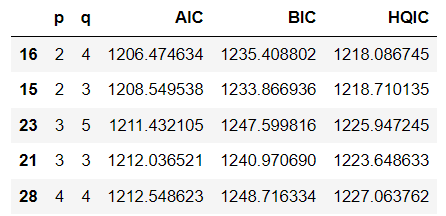
\includegraphics[width=10cm]{kryteria.png}
 	\caption{Indeksy poniżej -4 stopni zanotowane w 2015 roku}
 	
 \end{figure}

Najlepszymi parametrami okazuje się p = 2 oraz q = 4. Tych wartości użyjemy do estymacji parametrów modelu.\\
\newpage
Aby zmierzyć dopasowanie modelu najpierw sprawdźmy jak dopasował się on do danych treningowych za pomocą wykresu.\\

 \begin{figure}[h]
	
	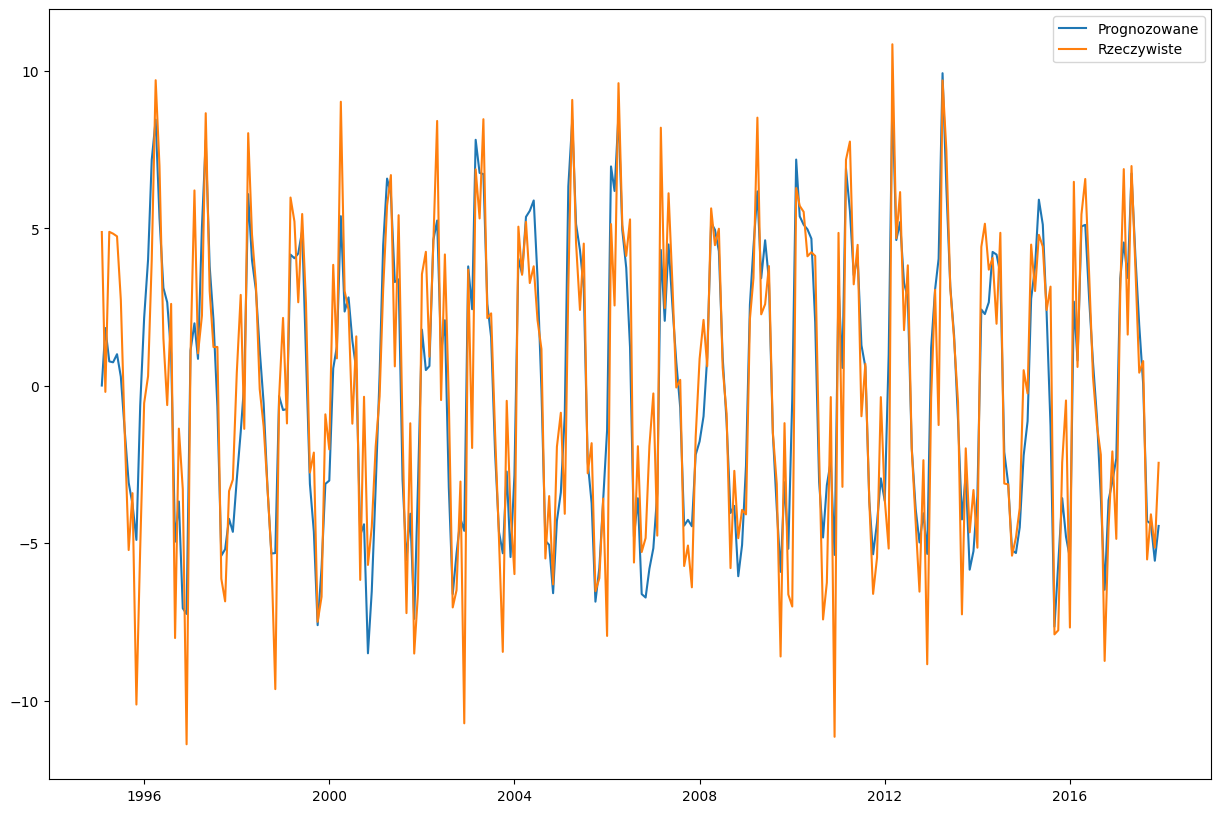
\includegraphics[width=10cm]{dopasowanie.png}
	\caption{Indeksy poniżej -4 stopni zanotowane w 2015 roku}
	
\end{figure}

Można zauważyć, że wartość niebieskie (prognozowane) mocno pokrywają się z wartościami rzeczywistymi. Oceńmy teraz dopasowanie do zbioru testowego.\\

 \begin{figure}[h]
	
	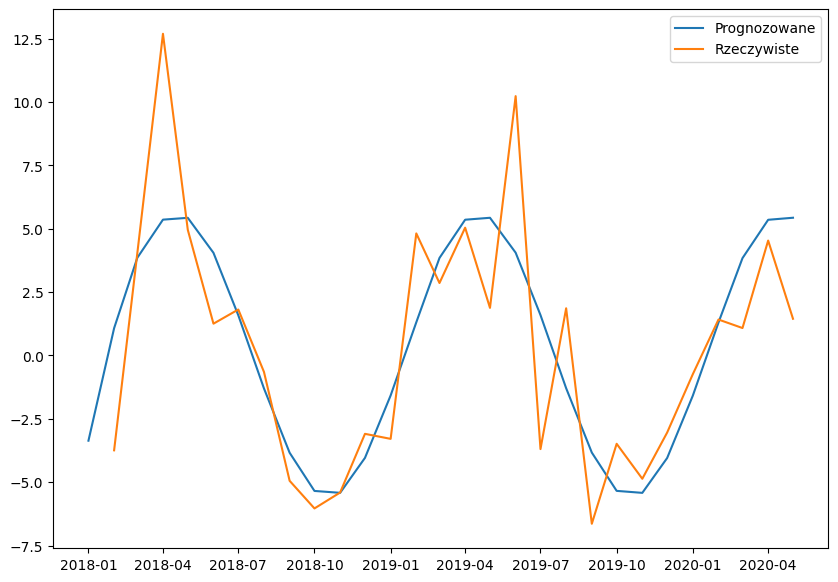
\includegraphics[width=10cm]{dopasowanie1.png}
	\caption{Indeksy poniżej -4 stopni zanotowane w 2015 roku}
	
\end{figure}

\newpage 

Wydaje się, że model ARMA w miare dobrze odwzorował wartości prognozowane. Za pomocą metryki $mean_absolute_percentage_error$ ocenimy dopasowanie modelu na zbiorze testowym oraz treningowym.\\

\begin{figure}[h]
	
	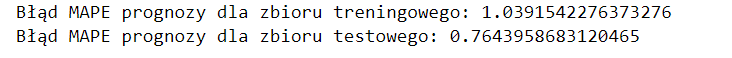
\includegraphics[width=10cm]{blad.png}
	\caption{Indeksy poniżej -4 stopni zanotowane w 2015 roku}
	
\end{figure}

Niższy błąd na zbiorze testowym (niż na treningowym) nie jest częstym przypadkiem. Przy klasycznych modelach uczenia maszynowego bardzo rzadko zdarza się taka sytuacja. Znacznie częsciej model notuje lepsze metryki na zbiorze, na którym się uczył. W naszej sytuacji jednak wynik jest inny, jest to oczywiście sytuacja dopuszczalna jednak nie zdarzająca się zbyt często. Błąd MAPE w okolicy 1 oznacza, że nasze wartości różnią się średnio o $1\%$ w stosunku do wartośći rzeczywistych. Jest to więc bardzo mały błąd.








	
\end{document}